\documentclass[12pt,a4paper]{article} % -*- latex -*-
\usepackage{geometry,amsmath}
\usepackage[utf8]{inputenc}
%\usepackage{xcolor}
\usepackage{color, colortbl}
\usepackage{amsfonts}
\definecolor{LRed}{rgb}{1,.8,.8}
\definecolor{MRed}{rgb}{1,.6,.6}
\definecolor{HRed}{rgb}{1,.2,.2}
\usepackage{tikz}
\usetikzlibrary{positioning,shapes,fit,arrows}
\definecolor{Gray}{gray}{0.9}
\definecolor{Green}{rgb}{0.3,0.9,0.3}
\definecolor{Red}{rgb}{0.98,0.3,0.3}
\usetikzlibrary{automata, positioning, arrows}
%Information to be included in the title page:

\tikzset{
        ->,  % makes the edges directed
        >=stealth', % makes the arrow heads boldnode 
        distance=3cm, % specifies the minimum distance between two nodes. Change if necessary.
        every state/.style={thick, fill=gray!10}, % sets the properties for each ’state’ node
        initial text=$ $, % sets the text that appears on the start arrow
}

\def\firstcircle{(90:1.75cm) circle (2cm)}
\def\secondcircle{(210:1.75cm) circle (2cm)}
\def\thirdcircle{(330:1.75cm) circle (2cm)}


\title{Exercise 4\\ Deep Learning}
\author{Dr. Mehrdad Maleki}
\date{Deadline: 19-June-2021}
\begin{document}
\maketitle
\begin{enumerate}

\item What is the Boolean gate for the $\overline{X}\vee Y$, i.e., find weights $w_1$, $w_2$ and bias $b$ such that the following gate model $\overline{X}\vee Y$,
\begin{center}
\begin{tikzpicture}
\draw[blue,ultra thick]  (3,0) circle (20pt);
\foreach \y in {2,-2}
  \draw[->] (0,\y) -- (2.3,0);
\foreach \y/\x in{2/$X$,-2/$Y$}
  \node[left] at (0,\y) {\x};

\foreach \y/\x in{2/$w_1$,-1.5/$w_2$}
  \node[above,orange] at (0+0.9,\y-0.5) {\x};

\draw[->] (3.7,0) -- (5,0);

\node[right,brown] at (5,0) {$\overline{X}\vee Y$};
\node[red] at (3,0) {$b$};
\end{tikzpicture}
\end{center}


\[
\overline{X} \vee Y=\left \{ \begin{array}{ll}
1 &\mbox{if }w_1X+w_2Y\geq b\\
0 &\mbox{else}
\end{array}
\right.
\]

\item What is the Boolean gate for the $X\wedge(Y\vee Z)$, i.e., find weights $w_1, w_2, w_3$ and bias $b$ such that the following gate model $X\wedge(Y\vee Z)$,
\begin{center}
\begin{tikzpicture}
\draw[blue,ultra thick]  (3,0) circle (20pt);
\foreach \y in {2,0,-2}
  \draw[->] (0,\y) -- (2.3,0);
\foreach \y/\x in{2/$X$,0/$Y$,-2/$Z$}
  \node[left] at (0,\y) {\x};

\foreach \y/\x in{2/$w_1$,0/$w_2$,-1.5/$w_3$}
  \node[above,orange] at (0+0.9,\y-0.5) {\x};

\draw[->] (3.7,0) -- (5,0);

\node[right,brown] at (5,0) {$X\wedge(Y\vee Z)$};
\node[red] at (3,0) {$b$};
\end{tikzpicture}
\end{center}


\[
X\wedge(Y\vee Z)=\left \{ \begin{array}{ll}
1 &\mbox{if }w_1X+w_2Y+w_3Z\geq b\\
0 &\mbox{else}
\end{array}
\right.
\]

\item You have been asked to design an image processing system that opens a gate when at least seven people are present in front of the gate. Your system can recognize maximum 50 people's faces with high accuracy. The main part of the system which is a Boolean gate will decide are there at least seven people in front of the gate? Complete the code below by fill in proper values for $w$ and $b$ to achieve this goal. Note that $gate(x)$ has to return $1$ for the given $x$ which represents the presence of people in front of the gate.

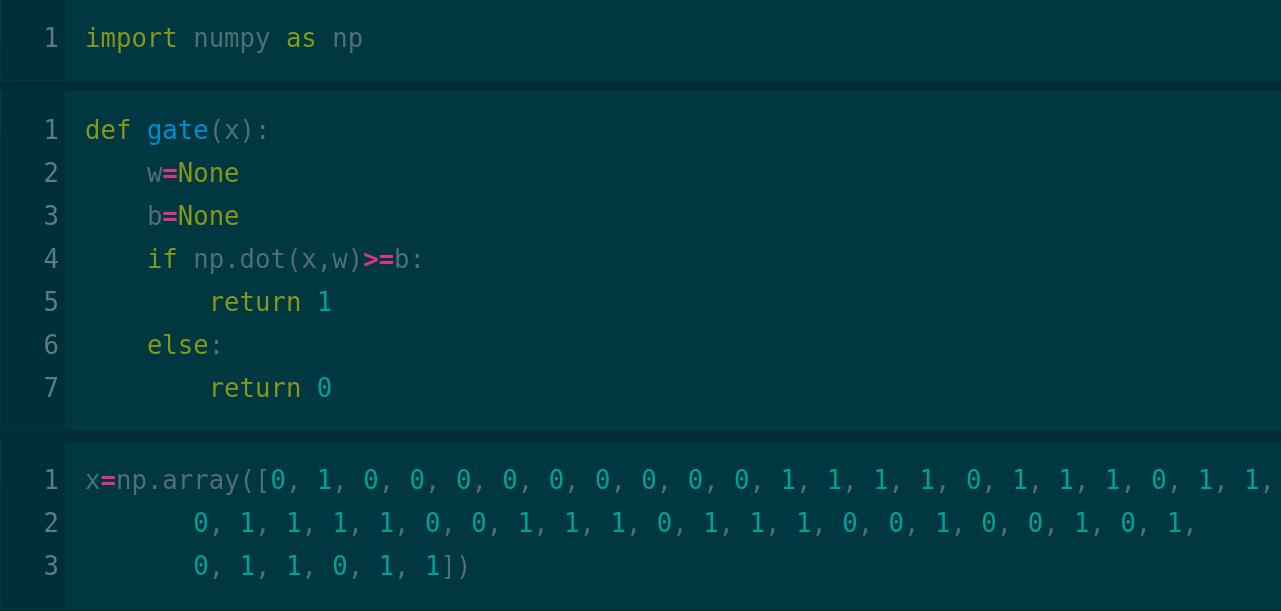
\includegraphics[scale=0.4]{ex4}

\end{enumerate}

\end{document}